\section{Experiments}
One of the most challenging aspects of developing image registration algorithms for brain MRI is validation. In order to rigorously evaluate the performance of non-linear
image registration algorithms, a ground-truth consisting of true correspondences between voxels of realistic pairs of images would be required. Since such a ground-truth data is
not currently available, researchers resort to surrogates that indirectly measure the quality of their algorithms. One of the most accepted surrogate measures is based
on the overlap of localized anatomical areas of registered images: ideally, corresponding anatomical areas of perfectly registered images should perfectly
overlap. Even a perfect registration algorithm is unlikely to achieve such an ambitious goal, though, since anatomical areas are usually defined manually by an expert, which is
by no means a perfect process and the annotations may vary even between different experts. Despite this limitation, it has been shown that among the alternative surrogate measures
usually employed, overlap scores of localized anatomical areas is the one that better distinguish reasonable from inaccurate registrations \cite{Rohlfing2012} and it has been employed
in the most rigorous evaluations of registration algorithms \cite{Klein2009}\cite{Klein2010}\cite{Rohlfing2012}. We also believe that rigorous reproducibility is of utmost importance. In our
experiments, we employ the publicly available IBSR database consisting of 18 manually annotated T1 brain MRI volumes, and made our algorithms also publicly available.

\subsection{Mono-modal registration}
Although our algorithms were designed for multi-modal image registration, it is important to first verify that the quality of the algorithms is reasonable for mono-modal registration.
Table \ref{tab:monomodal_results_seg} and figure \ref{fig:mono_graph_seg} show the average overlap score for each of 31 manually annotated anatomical regions from the IBSR database.
Note that the Jaccard indices obtained with the Cross Correlation metric (i.e. ANTS) are higher than reported by Rohlfing {\it et al.} \cite{Rohlfing2012}. In his experiments, he used
three resolutions with 10, 10 and 5 iterations only. Here, we used 100, 100 and 25 iterations, which stops the algorithm very close to convergence, leaving the rest of the parameters
unchanged. We can see that SyN with the EM metric is very competitive, but still not as good as Cross Correlation. This may be explained by the fact that CC uses a relatively large
window centered at each voxel for computing the similarity, while the EM is voxelwise. By considering neighborhoods of the same size, the Expected Cross Correlation metric performs
nearly as good as CC. Table \ref{tab:monomodal_results_segTri_fill} and figure \ref{fig:mono_graph_segTri_fill} show the overlap scores over tissue type, instead of anatomical areas.

% Table generated by Excel2LaTeX from sheet 'SyNEM-Monomodal-Large'
\begin{table}[p]
\begin{adjustwidth}{-0.75cm}{}
  {\centering
    \small
    \begin{tabular}{lcccc}
    \toprule
    \textbf{}& \textbf{SyN-EM} & \textbf{SyN-ECC} & \textbf{SyN-CC} & \textbf{SyN-MI} \\
    \midrule
    \textbf{Brain-Stem} & 0.786 & \textbf{0.816} & 0.812 & 0.804 \\
    \textbf{Right-Cerebellum-Cortex} & 0.736 & \textbf{0.815} & 0.813 & 0.771 \\
    \textbf{Left-Cerebellum-Cortex} & 0.739 & \textbf{0.811} & 0.808 & 0.766 \\
    \textbf{Right-Thalamus-Proper} & 0.714 & 0.766 & \textbf{0.772} & 0.745 \\
    \textbf{Left-Thalamus-Proper} & 0.727 & 0.763 & \textbf{0.767} & 0.748 \\
    \textbf{Right-Putamen} & 0.681 & 0.748 & \textbf{0.751} & 0.712 \\
    \textbf{Left-Putamen} & 0.699 & 0.744 & \textbf{0.744} & 0.721 \\
    \textbf{Left-Cerebral-Cortex} & 0.724 & \textbf{0.739} & 0.733 & 0.687 \\
    \textbf{Right-Cerebral-Cortex} & 0.719 & \textbf{0.739} & 0.731 & 0.683 \\
    \textbf{Right-Cerebral-White-Matter} & 0.702 & \textbf{0.733} & 0.720 & 0.645 \\
    \textbf{Left-Cerebral-White-Matter} & 0.705 & \textbf{0.732} & 0.721 & 0.646 \\
    \textbf{Left-Lateral-Ventricle} & 0.731 & 0.727 & \textbf{0.732} & 0.718 \\
    \textbf{Right-Lateral-Ventricle} & 0.709 & 0.714 & \textbf{0.717} & 0.699 \\
    \textbf{Right-Cerebellum-White-Matter} & 0.576 & \textbf{0.701} & 0.691 & 0.608 \\
    \textbf{Left-Cerebellum-White-Matter} & 0.581 & \textbf{0.701} & 0.693 & 0.611 \\
    \textbf{Left-Caudate} & 0.645 & \textbf{0.671} & 0.665 & 0.666 \\
    \textbf{Right-Caudate} & 0.620 & \textbf{0.655} & 0.647 & 0.651 \\
    \textbf{Right-VentralDC} & 0.612 & 0.651 & \textbf{0.652} & 0.628 \\
    \textbf{Left-VentralDC} & 0.622 & \textbf{0.651} & 0.650 & 0.631 \\
    \textbf{Right-Pallidum} & 0.498 & \textbf{0.622} & 0.620 & 0.582 \\
    \textbf{Right-Hippocampus} & 0.572 & \textbf{0.621} & 0.620 & 0.575 \\
    \textbf{Left-Pallidum} & 0.524 & \textbf{0.615} & 0.614 & 0.583 \\
    \textbf{Left-Hippocampus} & 0.574 & \textbf{0.610} & 0.609 & 0.564 \\
    \textbf{4th-Ventricle} & 0.551 & 0.606 & \textbf{0.608} & 0.574 \\
    \textbf{3rd-Ventricle} & 0.527 & 0.544 & \textbf{0.547} & 0.515 \\
    \textbf{Left-Amygdala} & 0.444 & 0.519 & \textbf{0.519} & 0.484 \\
    \textbf{Right-Amygdala} & 0.411 & 0.513 & \textbf{0.514} & 0.458 \\
    \textbf{Left-Accumbens-area} & 0.451 & 0.500 & \textbf{0.500} & 0.462 \\
    \textbf{Right-Accumbens-area} & 0.433 & 0.490 & \textbf{0.490} & 0.443 \\
    \textbf{Right-Inf-Lat-Vent} & 0.177 & 0.230 & \textbf{0.232} & 0.162 \\
    \textbf{Left-Inf-Lat-Vent} & 0.190 & 0.228 & \textbf{0.233} & 0.167 \\
    \hline
    \textbf{Average (std.)} & 0.593 (0.148) & 0.644 (0.142) & 0.643 (0.140) & 0.603 (0.149) \\
    \textbf{Rank-1 count} & 0 & 16 & 15 & 0 \\
    \textbf{Rank-2 count} & 1 & 14 & 14 & 2 \\
    \textbf{Rank-3 count} & 9 & 1 & 2 & 19 \\
    \bottomrule
    \end{tabular}}%
    \caption{Comparison of the registration performance (measured by the Jaccard index over 31 anatomical regions) of the Greedy SyN algorithm with EM, ECC, CC and MI metrics.
The Jaccard indices were averaged over 306 monomodal registrations. Rank-$k$ counts show the number of anatomical regions for which each
method ranked $k$ among the four methods under comparison. Top performer (rank-1) for each region is highlighted. }
  \label{tab:monomodal_results_seg}%
\end{adjustwidth}
\end{table}%

% Table generated by Excel2LaTeX from sheet 'SyNEM-Monomodal-Large'
\begin{table}[htbp]
  \centering
  {\small
    \begin{tabular}{rrrr}
    \toprule
    \textbf{} & \textbf{SyN-EM} & \textbf{SyN-ECC} & \textbf{SyN-CC} \\
    \midrule
    \textbf{Background} & 0.994 & 0.995 & \textbf{0.995} \\
    \textbf{CSF} & 0.335 & 0.349 & \textbf{0.359} \\
    \textbf{Gray Matter} & 0.740 & \textbf{0.765} & 0.759 \\
    \textbf{White Matter} & 0.703 & \textbf{0.739} & 0.728 \\
    \bottomrule
    \end{tabular}%
    \caption{Comparison of the registration performance (measured by the Jaccard index over Background, CSF, GM and WM)of the Greedy SyN algorithm with EM, ECC and CC metrics. The Jaccard
indices were averaged over 306 monomodal registrations. Top performer for each region is highlighted.}
  \label{tab:monomodal_results_segTri_fill}}%
\end{table}%


\begin{figure}[H]
\centering
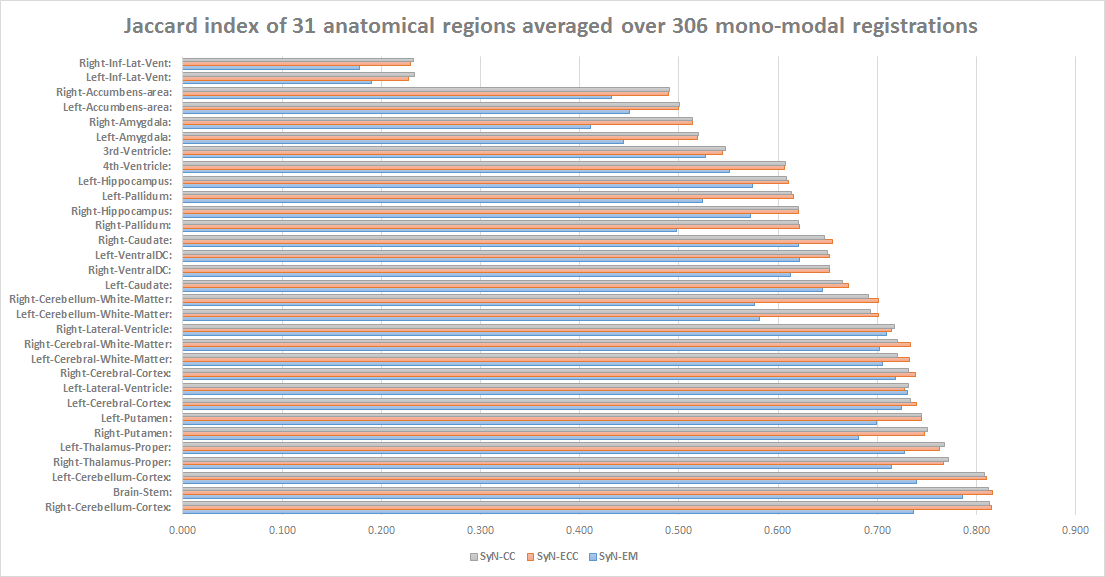
\includegraphics[width=1.0\linewidth]{./images/mono_graph_seg.png}\\
\caption{Comparison of the registration performance (measured by the Jaccard index over 31 anatomical regions) of the Greedy SyN algorithm with EM, ECC and CC metrics. The Jaccard
indices were averaged over 306 monomodal registrations.}
\label{fig:mono_graph_seg}
\end{figure}

\begin{figure}[H]
\centering
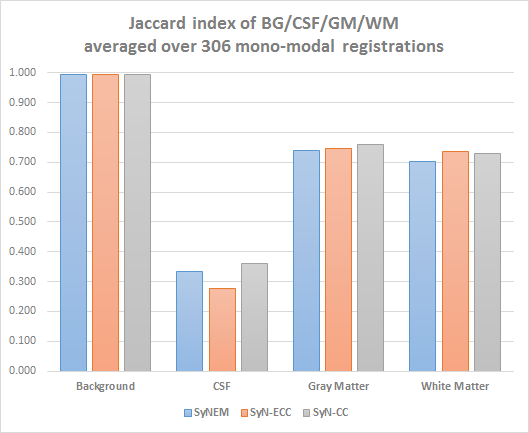
\includegraphics[width=0.5\linewidth]{./images/mono_graph_segTri_fill.png}\\
\caption{Comparison of the registration performance (measured by the Jaccard index over Background, CSF, GM and WM)of the Greedy SyN algorithm with EM, ECC and CC metrics. The Jaccard
indices were averaged over 306 monomodal registrations.}
\label{fig:mono_graph_segTri_fill}
\end{figure}


\subsection{Multi-modal registration}
It is a common practice within the neuroimaging community to use the cross-correlation metric to register T1 vs T2 brain MRI images. The argument in favor of using
this metric is that these modalities are related by an ``almost linear'' transfer function. To illustrate the danger of doing this, we used the Brainweb synthetic
template \cite{Cocosco1997}\cite{Kwan1999}. Brainweb provides two perfectly aligned, realistically simulated brain MRI in T1 and T2 modalities
(fig. \ref{fig:brainweb_t1_t2_input}). Ideally, a multi-modal registration method should return the identity transformation to register these perfectly aligned images.
Figure \ref{fig:syncc_brainweb_t1_t2_overlay} depicts the result of registering the images using ANTS with the Cross Correlation metric. We can see that the cortex was
(incorrectly) strongly deformed: the deformation field maximizing the cross correlation between the two multi-modal images does not coincides with the deformation field
correctly aligning the images. Figure \ref{fig:syencc_brainweb_t1_t2_overlay} depicts the result of registering the images using the Expected Cross-Correlation metric.
Although the deformation field is not exactly zero, the deformations are much smaller.

\begin{figure}[H]
\centering
\fbox{\subfloat[Brainweb T1 (left) and T2(right) overlaid using two different channels(middle). T1 is depicted in red and T2 in green.]{\label{fig:brainweb_t1_t2_input}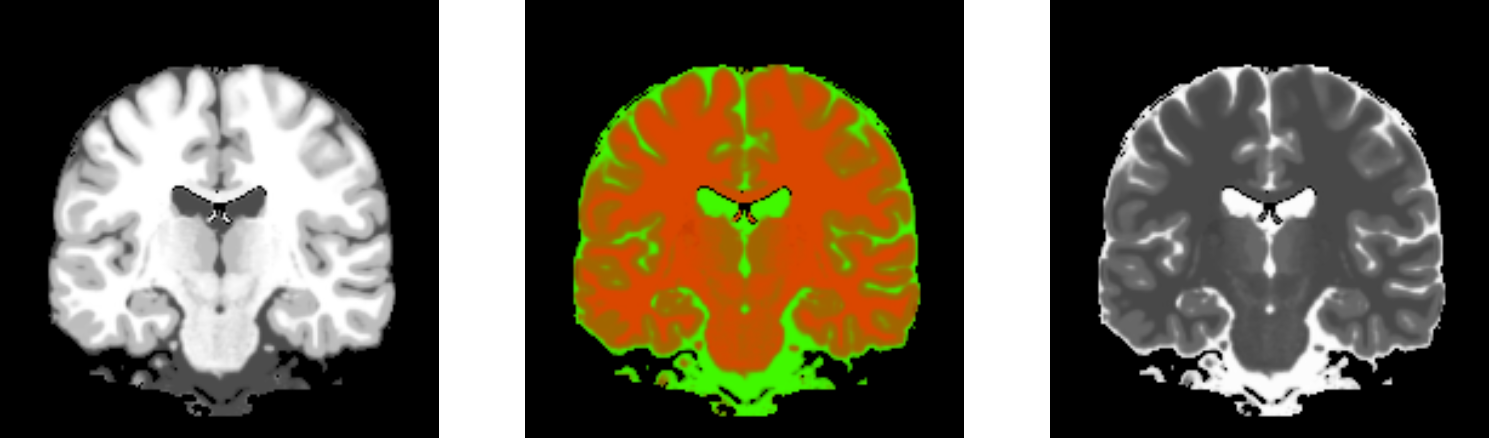
\includegraphics[width=1.0\linewidth]{./images/brainweb_t1_t2_overlay.png}}}\\
\fbox{\subfloat[T2 registered towards T1 using ANTS with the Cross-Correlation metric. Boundaries are clearly distorted.]{\label{fig:syncc_brainweb_t1_t2_overlay}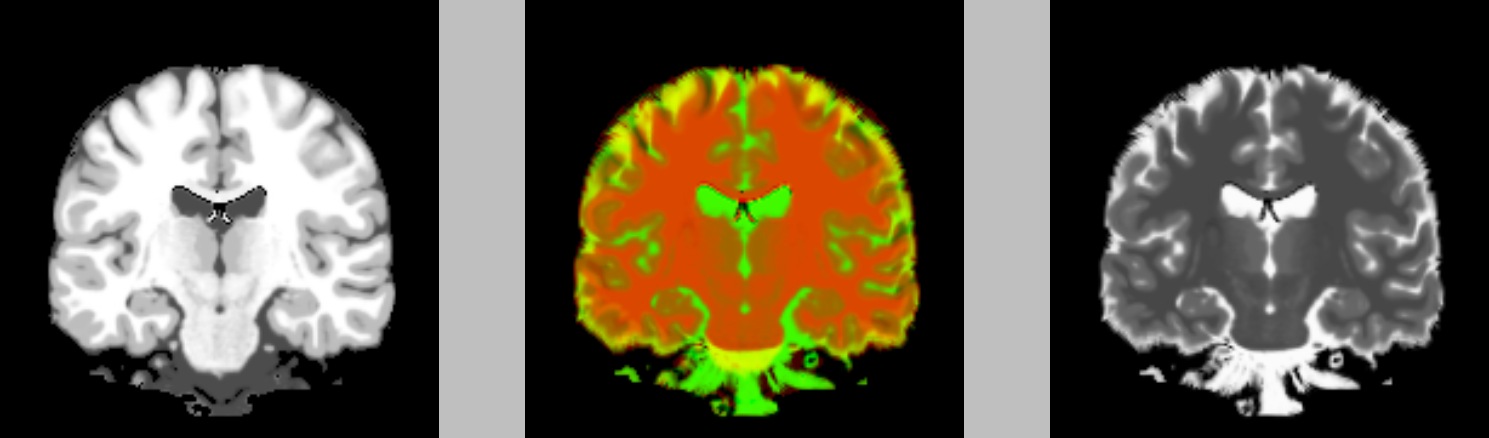
\includegraphics[width=1.0\linewidth]{./images/syncc_brainweb_t1_t2_overlay.png}}}\\
\fbox{\subfloat[T2 registered towards T1 using SyN algorithm with the Expected Cross-Correlation metric. Deformations are hard to see: ventricles are slightly dilated.]{\label{fig:syencc_brainweb_t1_t2_overlay}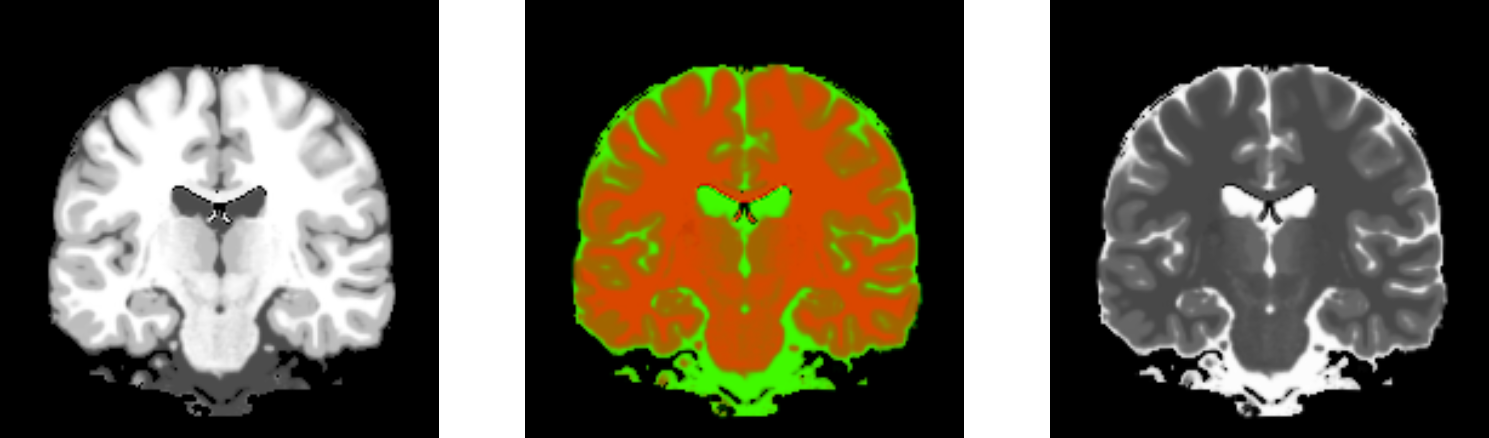
\includegraphics[width=1.0\linewidth]{./images/synecc_brainweb_t1_t2_overlay.png}}}\\
\fbox{\subfloat[Norm of displacement vectors obtained with the ECC metric. The average norm was 0.26 voxels (excluding background voxels) with a maximum of 2.6 voxels. \textcolor{red}{TO-DO: correct the incorrectly excluded voxels inside the brain(it's CSF, not BG)}]{\label{fig:synecc_disp_norms}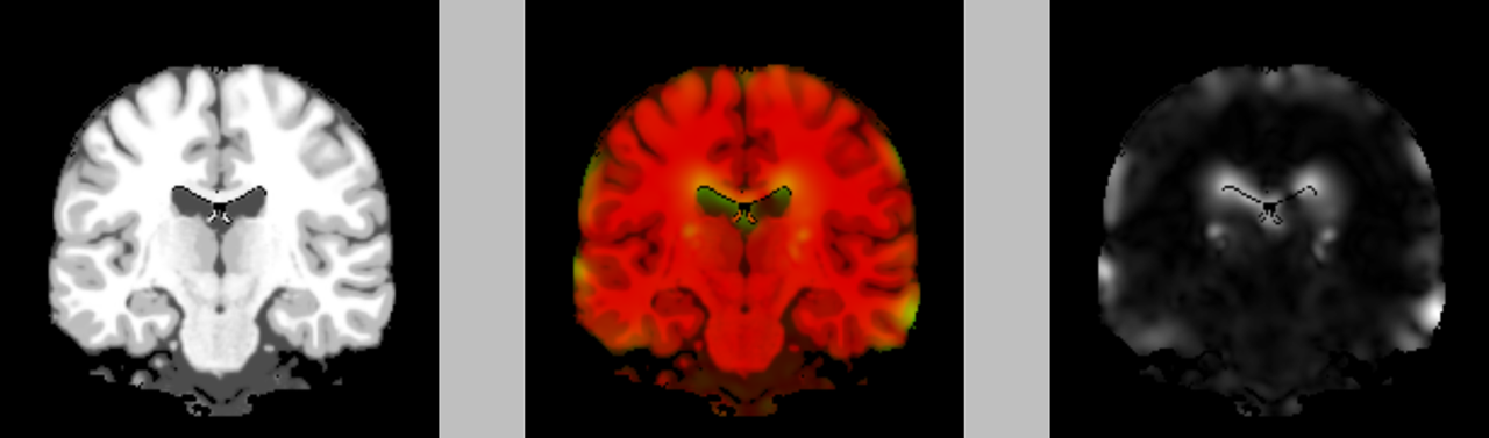
\includegraphics[width=1.0\linewidth]{./images/synecc_disp_norms.png}}}
\caption{Registration of two perfectly aligned images with different modalities.}
\label{fig:brainweb_t1_t2}
\end{figure}

The above experiment is hardly a compelling evidence that the ECC metric performs better than CC for multi-modal registration. Unfortunately, to the best of our knowledge,
there are no manually annotated multi-modality data publicly available, so we will perform a less
realistic experiment using the Brainweb template. We generated synthetic T2 images for all IBSR T1 images by first registering the Brainweb T1 image (which plays the role of
moving image) towards each IBSR T1 image (which play the role of static image) using ANTS. Then we applied the obtained deformation field to the Brainweb T2 image and computed
the transfer function from T1 to T2 intensities and applied the transfer function to the IBSR T1 obtaining a ``perfectly aligned'' realistic synthetic T2 image for each IBSR volume
(fig. \ref{fig:semi_synthetic}), therefore the annotations remain exactly the same as the T1 counterparts and we are able to compute the overlap scores as before. Note that the number
of registrations we need to perform is now 612 because we can use the T2 modality either as the moving or the static image. Table \ref{tab:multimodal_results_seg} and
figure \ref{fig:multi_graph_seg} show the results analogous to table \ref{tab:monomodal_results_seg} and figure \ref{fig:mono_graph_seg} but this time averaged over 612
multimodal registrations. Note how the performance of the CC metric strongly drops while EM and ECC are less affected by the change of modality. Table
\ref{tab:multimodal_results_segTri_fill} and figure \ref{fig:multi_graph_segTri_fill} show the overlap scores of tissue types, where the same
behavior can be observed.\\

\begin{figure}[H]
\centering
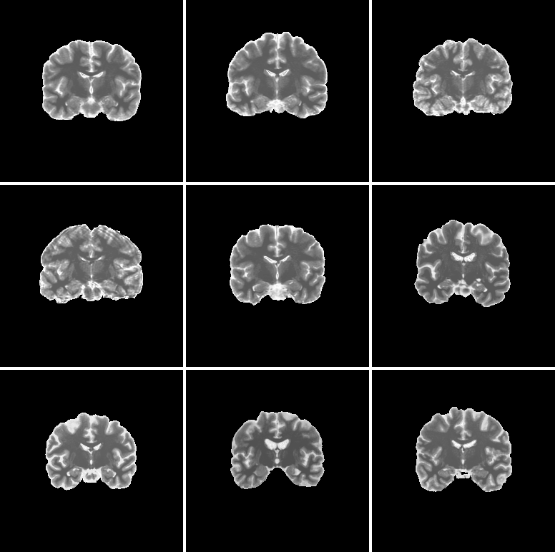
\includegraphics[width=1.0\linewidth]{./images/semi_synthetic.png}\\
\caption{First 9 T2 images generated from the real IBSR T1 images and the T2 Brainweb template (see text). Since the anatomy remained unchanged, the manual annotations are exactly
the same as the corresponding T1 images.}
\label{fig:semi_synthetic}
\end{figure}

% Table generated by Excel2LaTeX from sheet 'SyNEM-Multi-Large'
\begin{table}[htbp]
  \centering
  {\small
    \begin{tabular}{rrrr}
    \toprule
          & \textbf{SyN-ECC} & \textbf{SyN-EM} & \textbf{SyN-CC} \\
    \midrule
    \textbf{Right-Thalamus-Proper:} & \textbf{0.758} & 0.716 & 0.756 \\
    \textbf{Left-Thalamus-Proper:} & \textbf{0.754} & 0.727 & 0.752 \\
    \textbf{Left-Lateral-Ventricle:} & 0.709 & 0.706 & \textbf{0.733} \\
    \textbf{Right-Lateral-Ventricle:} & 0.696 & 0.687 & \textbf{0.718} \\
    \textbf{Left-Putamen:} & \textbf{0.740} & 0.699 & 0.683 \\
    \textbf{Right-Putamen:} & \textbf{0.742} & 0.684 & 0.676 \\
    \textbf{Brain-Stem:} & \textbf{0.790} & 0.786 & 0.663 \\
    \textbf{Left-Cerebellum-Cortex:} & \textbf{0.765} & 0.729 & 0.649 \\
    \textbf{Right-Cerebellum-Cortex:} & \textbf{0.769} & 0.729 & 0.645 \\
    \textbf{Left-Caudate:} & \textbf{0.652} & 0.628 & 0.637 \\
    \textbf{Right-Caudate:} & \textbf{0.636} & 0.606 & 0.618 \\
    \textbf{Right-Cerebral-White-Matter:} & \textbf{0.723} & 0.683 & 0.571 \\
    \textbf{Left-Cerebral-White-Matter:} & \textbf{0.722} & 0.685 & 0.570 \\
    \textbf{Left-Cerebral-Cortex:} & \textbf{0.700} & 0.699 & 0.558 \\
    \textbf{Right-Cerebral-Cortex:} & \textbf{0.697} & 0.694 & 0.548 \\
    \textbf{4th-Ventricle:} & \textbf{0.583} & 0.546 & 0.543 \\
    \textbf{Right-Hippocampus:} & \textbf{0.610} & 0.570 & 0.503 \\
    \textbf{Right-VentralDC:} & \textbf{0.642} & 0.616 & 0.499 \\
    \textbf{Right-Pallidum:} & \textbf{0.606} & 0.528 & 0.499 \\
    \textbf{Left-Pallidum:} & \textbf{0.602} & 0.545 & 0.495 \\
    \textbf{3rd-Ventricle:} & \textbf{0.517} & 0.511 & 0.492 \\
    \textbf{Left-VentralDC:} & \textbf{0.640} & 0.622 & 0.491 \\
    \textbf{Left-Hippocampus:} & \textbf{0.600} & 0.567 & 0.488 \\
    \textbf{Left-Cerebellum-White-Matter:} & \textbf{0.688} & 0.582 & 0.485 \\
    \textbf{Right-Cerebellum-White-Matter:} & \textbf{0.690} & 0.579 & 0.476 \\
    \textbf{Left-Amygdala:} & \textbf{0.505} & 0.447 & 0.360 \\
    \textbf{Right-Amygdala:} & \textbf{0.497} & 0.415 & 0.339 \\
    \textbf{Right-Accumbens-area:} & \textbf{0.483} & 0.433 & 0.339 \\
    \textbf{Left-Accumbens-area:} & \textbf{0.494} & 0.448 & 0.338 \\
    \textbf{Left-Inf-Lat-Vent:} & \textbf{0.219} & 0.178 & 0.194 \\
    \textbf{Right-Inf-Lat-Vent:} & \textbf{0.219} & 0.164 & 0.178 \\
    \bottomrule
    \end{tabular}}%
    \caption{Comparison of the registration performance (measured by the Jaccard index over 31 anatomical regions) of the Greedy SyN algorithm with EM, ECC and CC metrics. The Jaccard
indices were averaged over 612 multimodal registrations. Top performer for each region is highlighted.}
  \label{tab:multimodal_results_seg}%
\end{table}%

% Table generated by Excel2LaTeX from sheet 'SyNEM-Multi-Large'
\begin{table}[htbp]
  \centering
  {\small
    \begin{tabular}{ccccc}
    \toprule
          & \textbf{SyN-EM} & \textbf{SyN-ECC} & \textbf{SyN-CC} & \textbf{SyN-MI} \\
    \midrule
    \textbf{Background} & 0.993 & 0.995 & 0.990 & \textbf{0.995} \\
    \textbf{CSF} & 0.275 & \textbf{0.335} & 0.157 & 0.325 \\
    \textbf{Gray Matter} & 0.718 & \textbf{0.742} & 0.597 & 0.691 \\
    \textbf{White Matter} & 0.685 & \textbf{0.718} & 0.572 & 0.622 \\
    \bottomrule
    \end{tabular}}%
  \caption{Comparison of the registration performance (measured by the Jaccard index over Background, CSF, GM and WM)of the Greedy SyN algorithm with EM, ECC, CC and MI metrics.
The Jaccard indices were averaged over 612 multimodal registrations. Top performer for each region is highlighted.}
  \label{tab:multimodal_results_segTri_fill}%
\end{table}%


\begin{figure}[H]
\centering
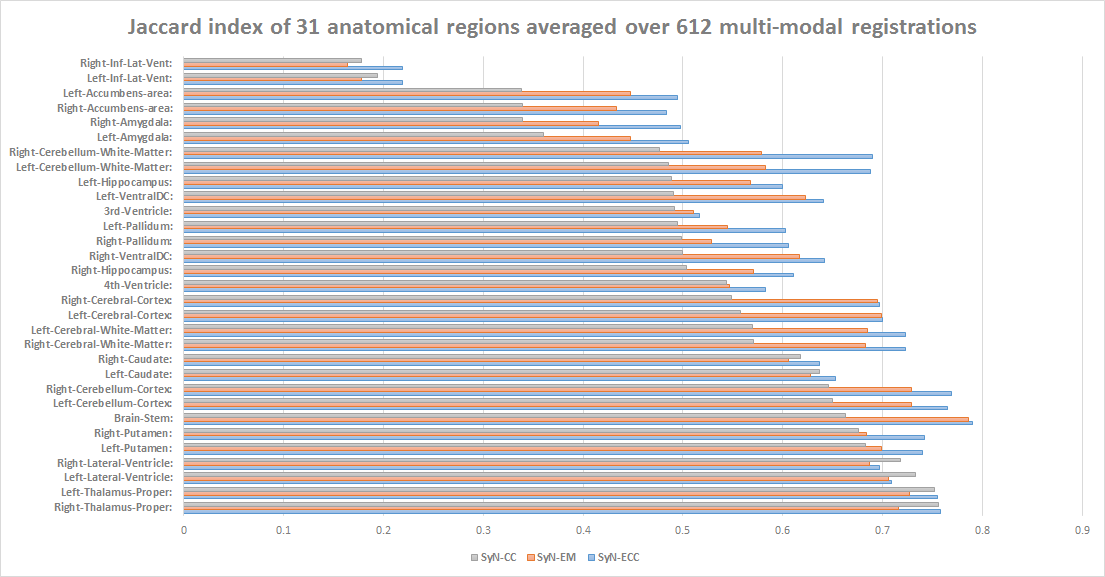
\includegraphics[width=1.0\linewidth]{./images/multi_graph_seg.png}\\
\caption{Comparison of the registration performance (measured by the Jaccard index over 31 anatomical regions) of the Greedy SyN algorithm with EM, ECC and CC metrics. The Jaccard
indices were averaged over 612 multimodal registrations.}
\label{fig:multi_graph_seg}
\end{figure}

\begin{figure}[H]
\centering
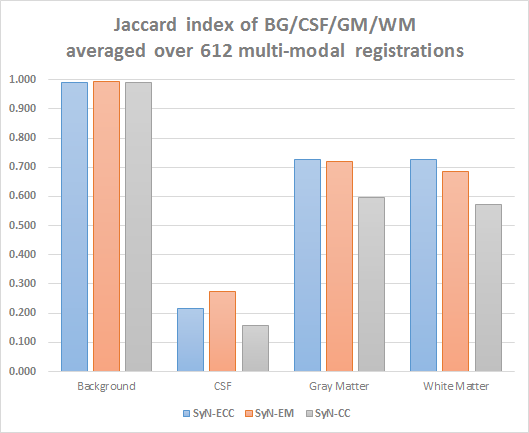
\includegraphics[width=0.5\linewidth]{./images/multi_graph_segTri_fill.png}\\
\caption{Comparison of the registration performance (measured by the Jaccard index over Background, CSF, GM and WM)of the Greedy SyN algorithm with EM, ECC and CC metrics. The Jaccard
indices were averaged over 612 multimodal registrations.}
\label{fig:multi_graph_segTri_fill}
\end{figure}
